\documentclass{beamer}

\mode<presentation>{\usetheme{Madrid}}
\usepackage{graphicx}
\usepackage{multimedia}
\usepackage{hyperref}

\usepackage[utf8]{inputenc}
\usepackage[ngerman]{babel}
\usepackage{amsmath, amssymb, amsthm}

\usepackage{subcaption}
\usepackage[T1]{fontenc}
%\usepackage[sort&compress]{natbib}

\usepackage{lmodern}
\usepackage{caption}


\author[Jan Niclas Ruppenthal, Michael Feldmann, Philipp Geier]{}
\title[]{3. Übung zur Vorlesung
Virtual Reality\\ Embodied Locomotion}
\institute[Universität Trier]{}
\date[10. Juni 2024]{}
\beamertemplatenavigationsymbolsempty
\setbeamertemplate{footline}
{
  \leavevmode%
  \hbox{%
  \begin{beamercolorbox}[wd=.50\paperwidth,ht=2.25ex,dp=1ex,center]{author in head/foot}%
    \usebeamerfont{author in head/foot}\insertshortauthor%~~\beamer@ifempty{\insertshortinstitute}{}{(\insertshortinstitute)}
  \end{beamercolorbox}%
  \begin{beamercolorbox}[wd=.50\paperwidth,ht=2.25ex,dp=1ex,right]{date in head/foot}%
    \usebeamerfont{date in head/foot}\insertshortdate{}\hspace*{2em}
    \insertframenumber{} / \inserttotalframenumber\hspace*{2ex} 
  \end{beamercolorbox}}%
  \vskip0pt%
}
%—-------------------------------------------------------------

\begin{document}
{
  \usebackgroundtemplate{
    \hspace{1.8cm} 
\includegraphics[width=.8\paperwidth]{img/cop}}
  \begin{frame}
    \maketitle
  \end{frame}
}
    
    %\begin{frame}
       % \frametitle{Inhalt}
		%\tableofcontents
	%\end{frame}
	
%—------------------------------------------------------


\begin{frame}{Locomotion}
\begin{figure}
    \centering
    \movie[externalviewer]{
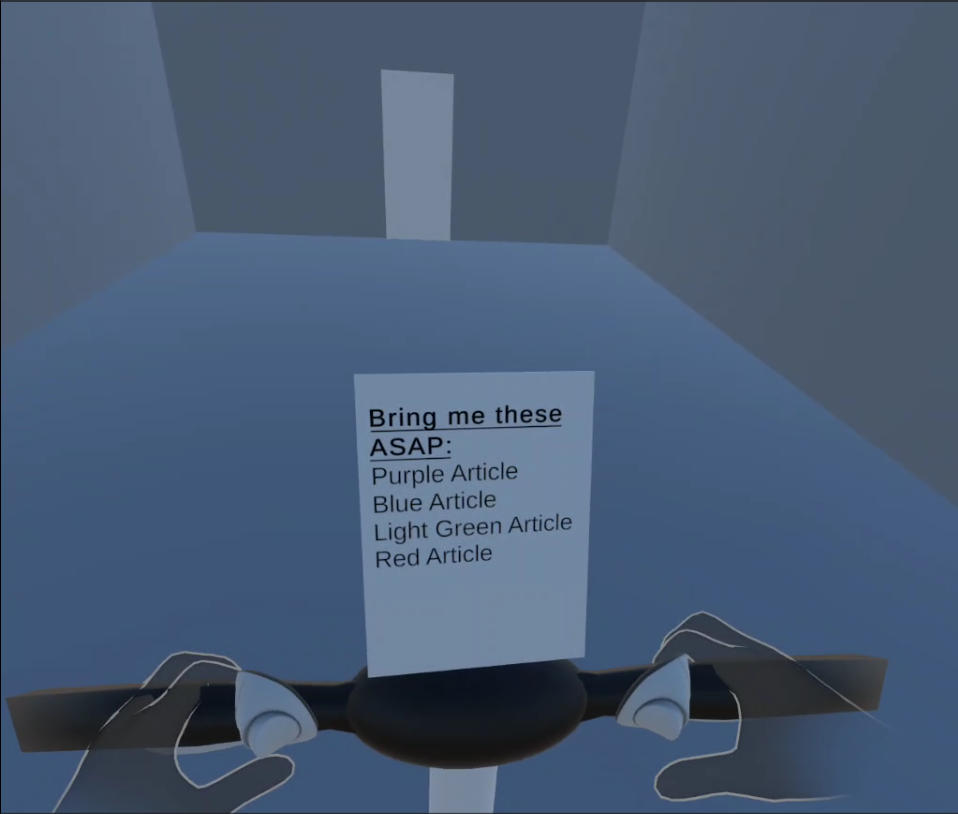
\includegraphics[width=0.6\textwidth, keepaspectratio]{img/Locomotion}
}{vid/Locomotion_Movement.mp4}
\caption{Locomotion}
\end{figure}
\end{frame}

\begin{frame}{Locomotion}
\textbf{Metapher}
\begin{itemize}
\item Steering-Leaning:\begin{itemize}
\item 1 DOF vTranslation: Durch Lehnen entlang der z-Achse
\item 1 DOF vRotation: Durch Bewegen der Controller entlang der x-Achse
\end{itemize}
\end{itemize}
\textbf{Travel-Task}
\begin{itemize}
\item Search
\end{itemize}
\end{frame}

\begin{frame}{Locomotion}
\textbf{Funktion}
\begin{itemize}
\item Leaning:\begin{itemize}
\item Powerfunktion mit Deadzone von 5 cm
\item Maximalgeschwindigkeit: 5 Meter pro Sekunde nach 34.8 cm
\end{itemize}
\end{itemize}
\begin{figure}
\centering
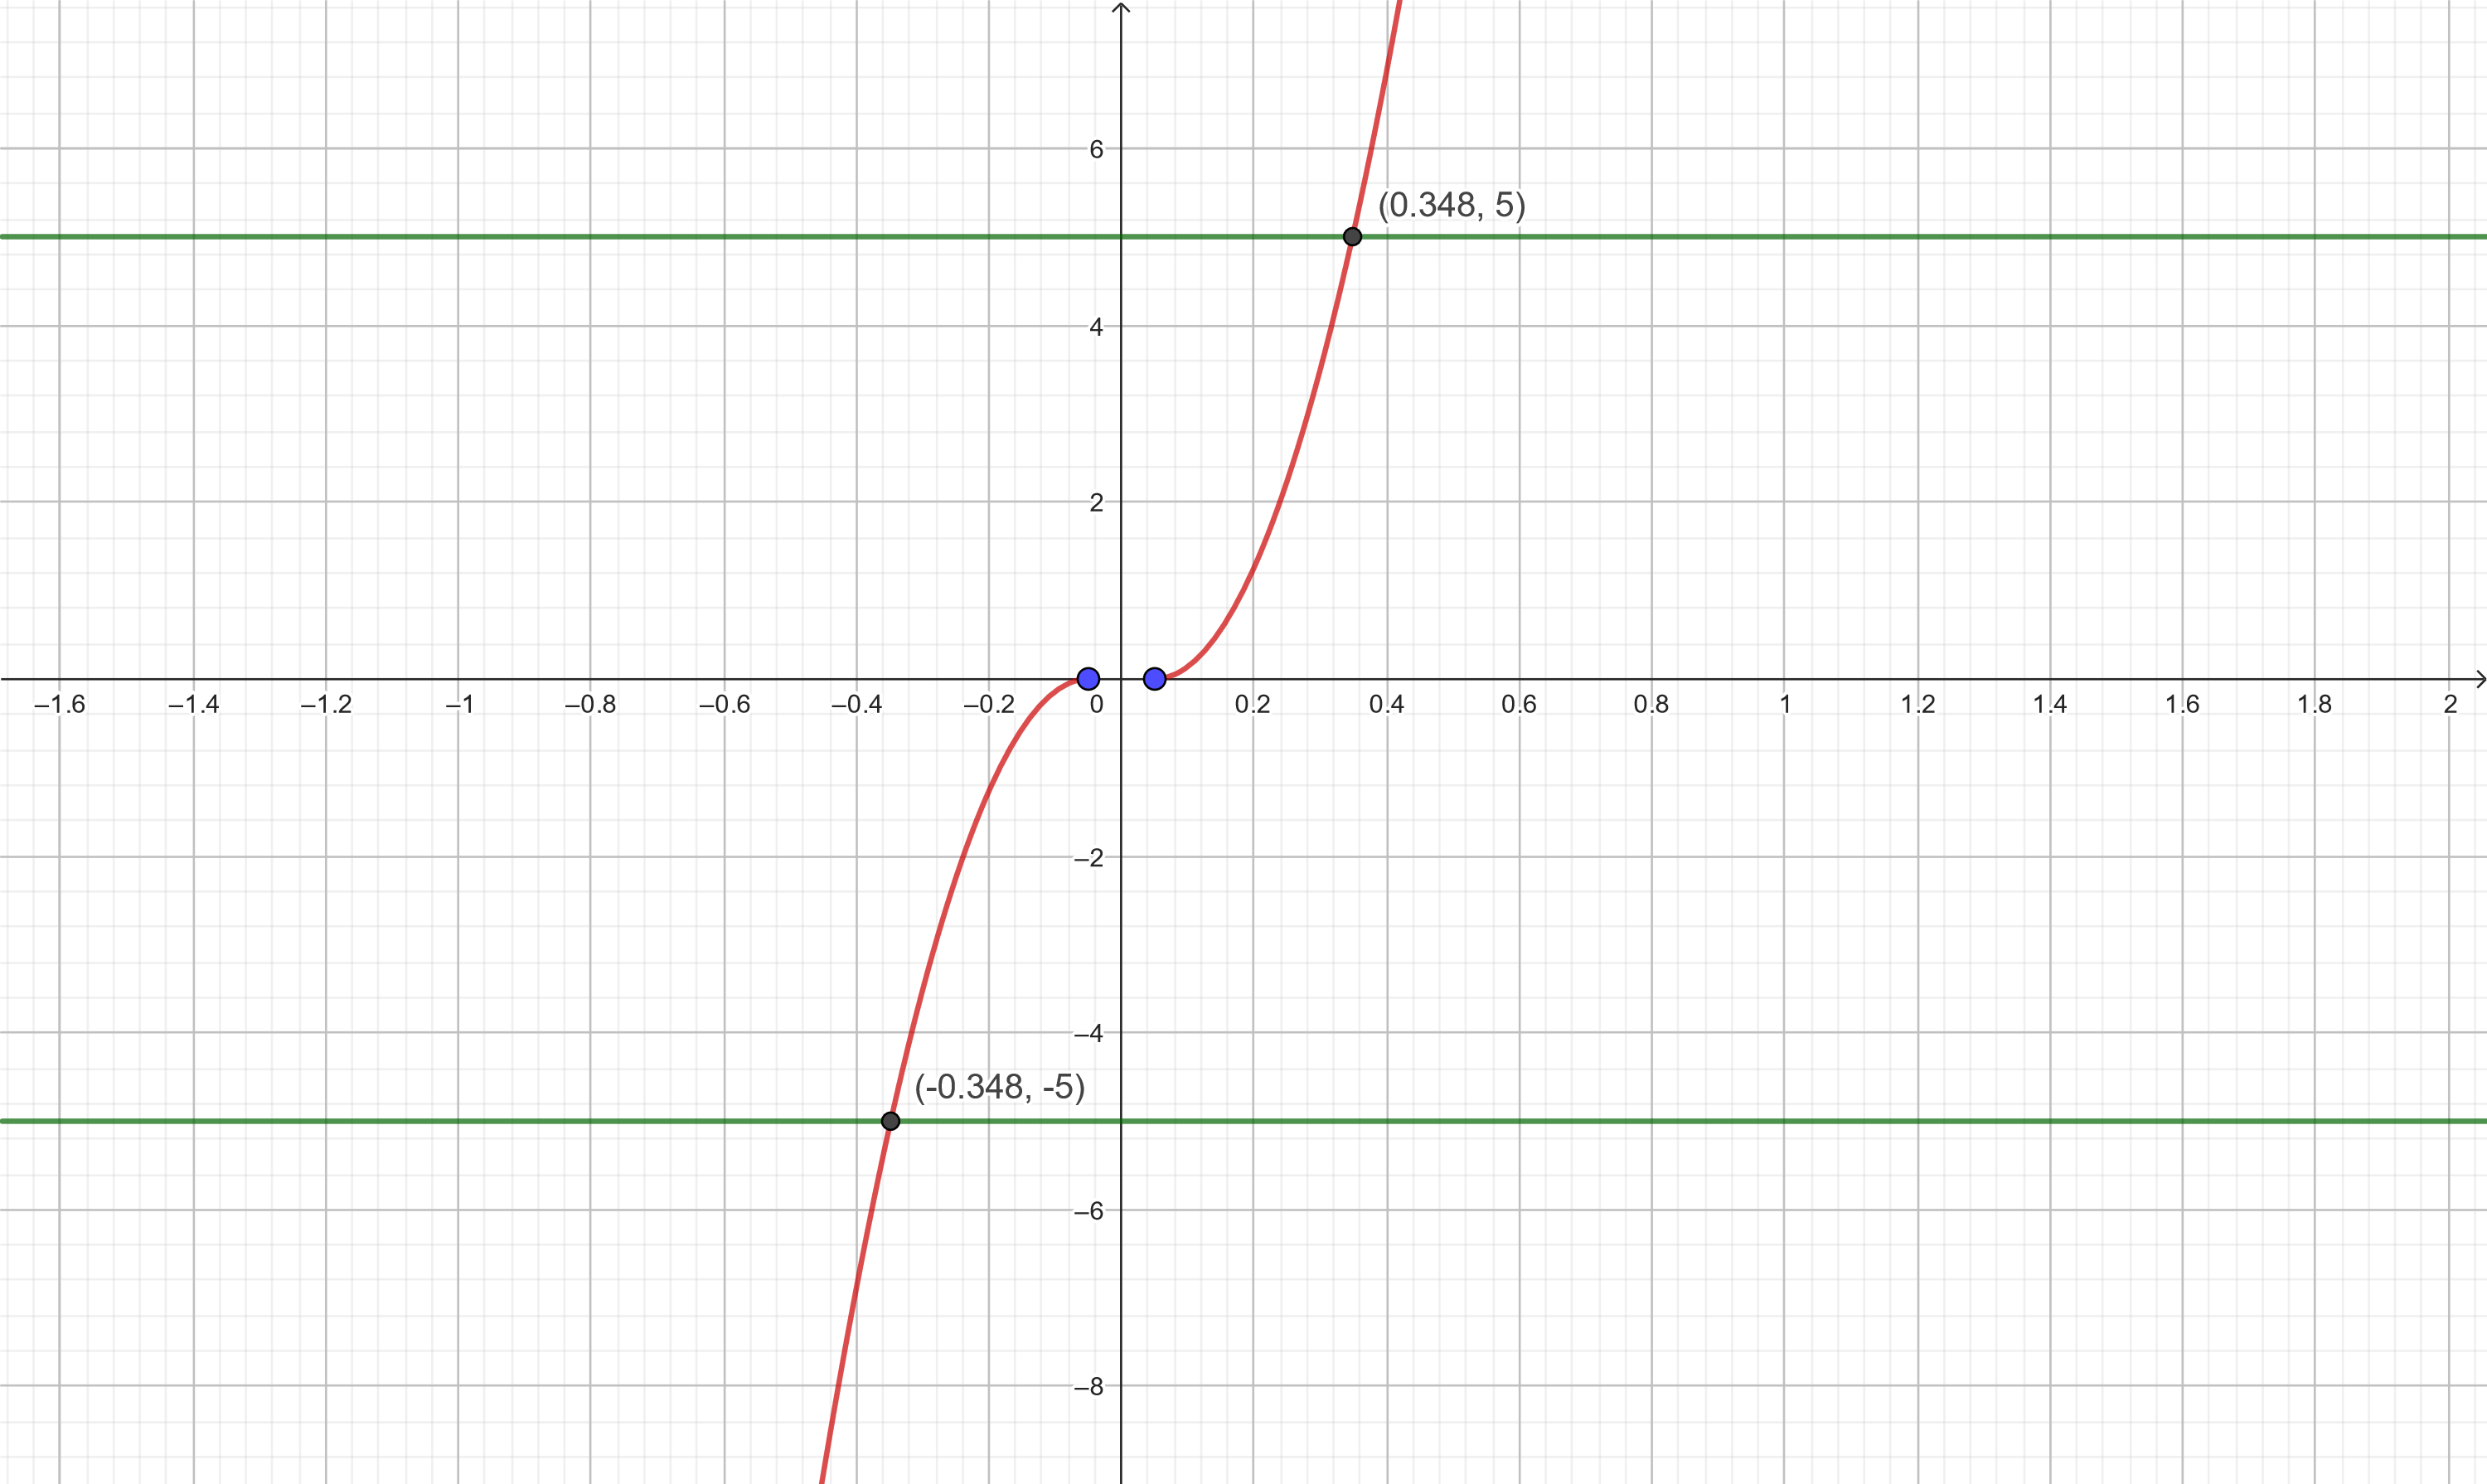
\includegraphics[width=.7\textwidth, keepaspectratio]{img/Movement}
\caption{Movement}
\end{figure}
\end{frame}

\begin{frame}{Locomotion}
\textbf{Funktion}
\begin{itemize}
\item Steering:\begin{itemize}
\item Funktion: Powerfunktion mit Deadzone von 10 cm
\item Maximalgeschwindigkeit: 30 Grad pro Sekunde nach 28.3 cm
\end{itemize}
\end{itemize}
\begin{figure}
\centering
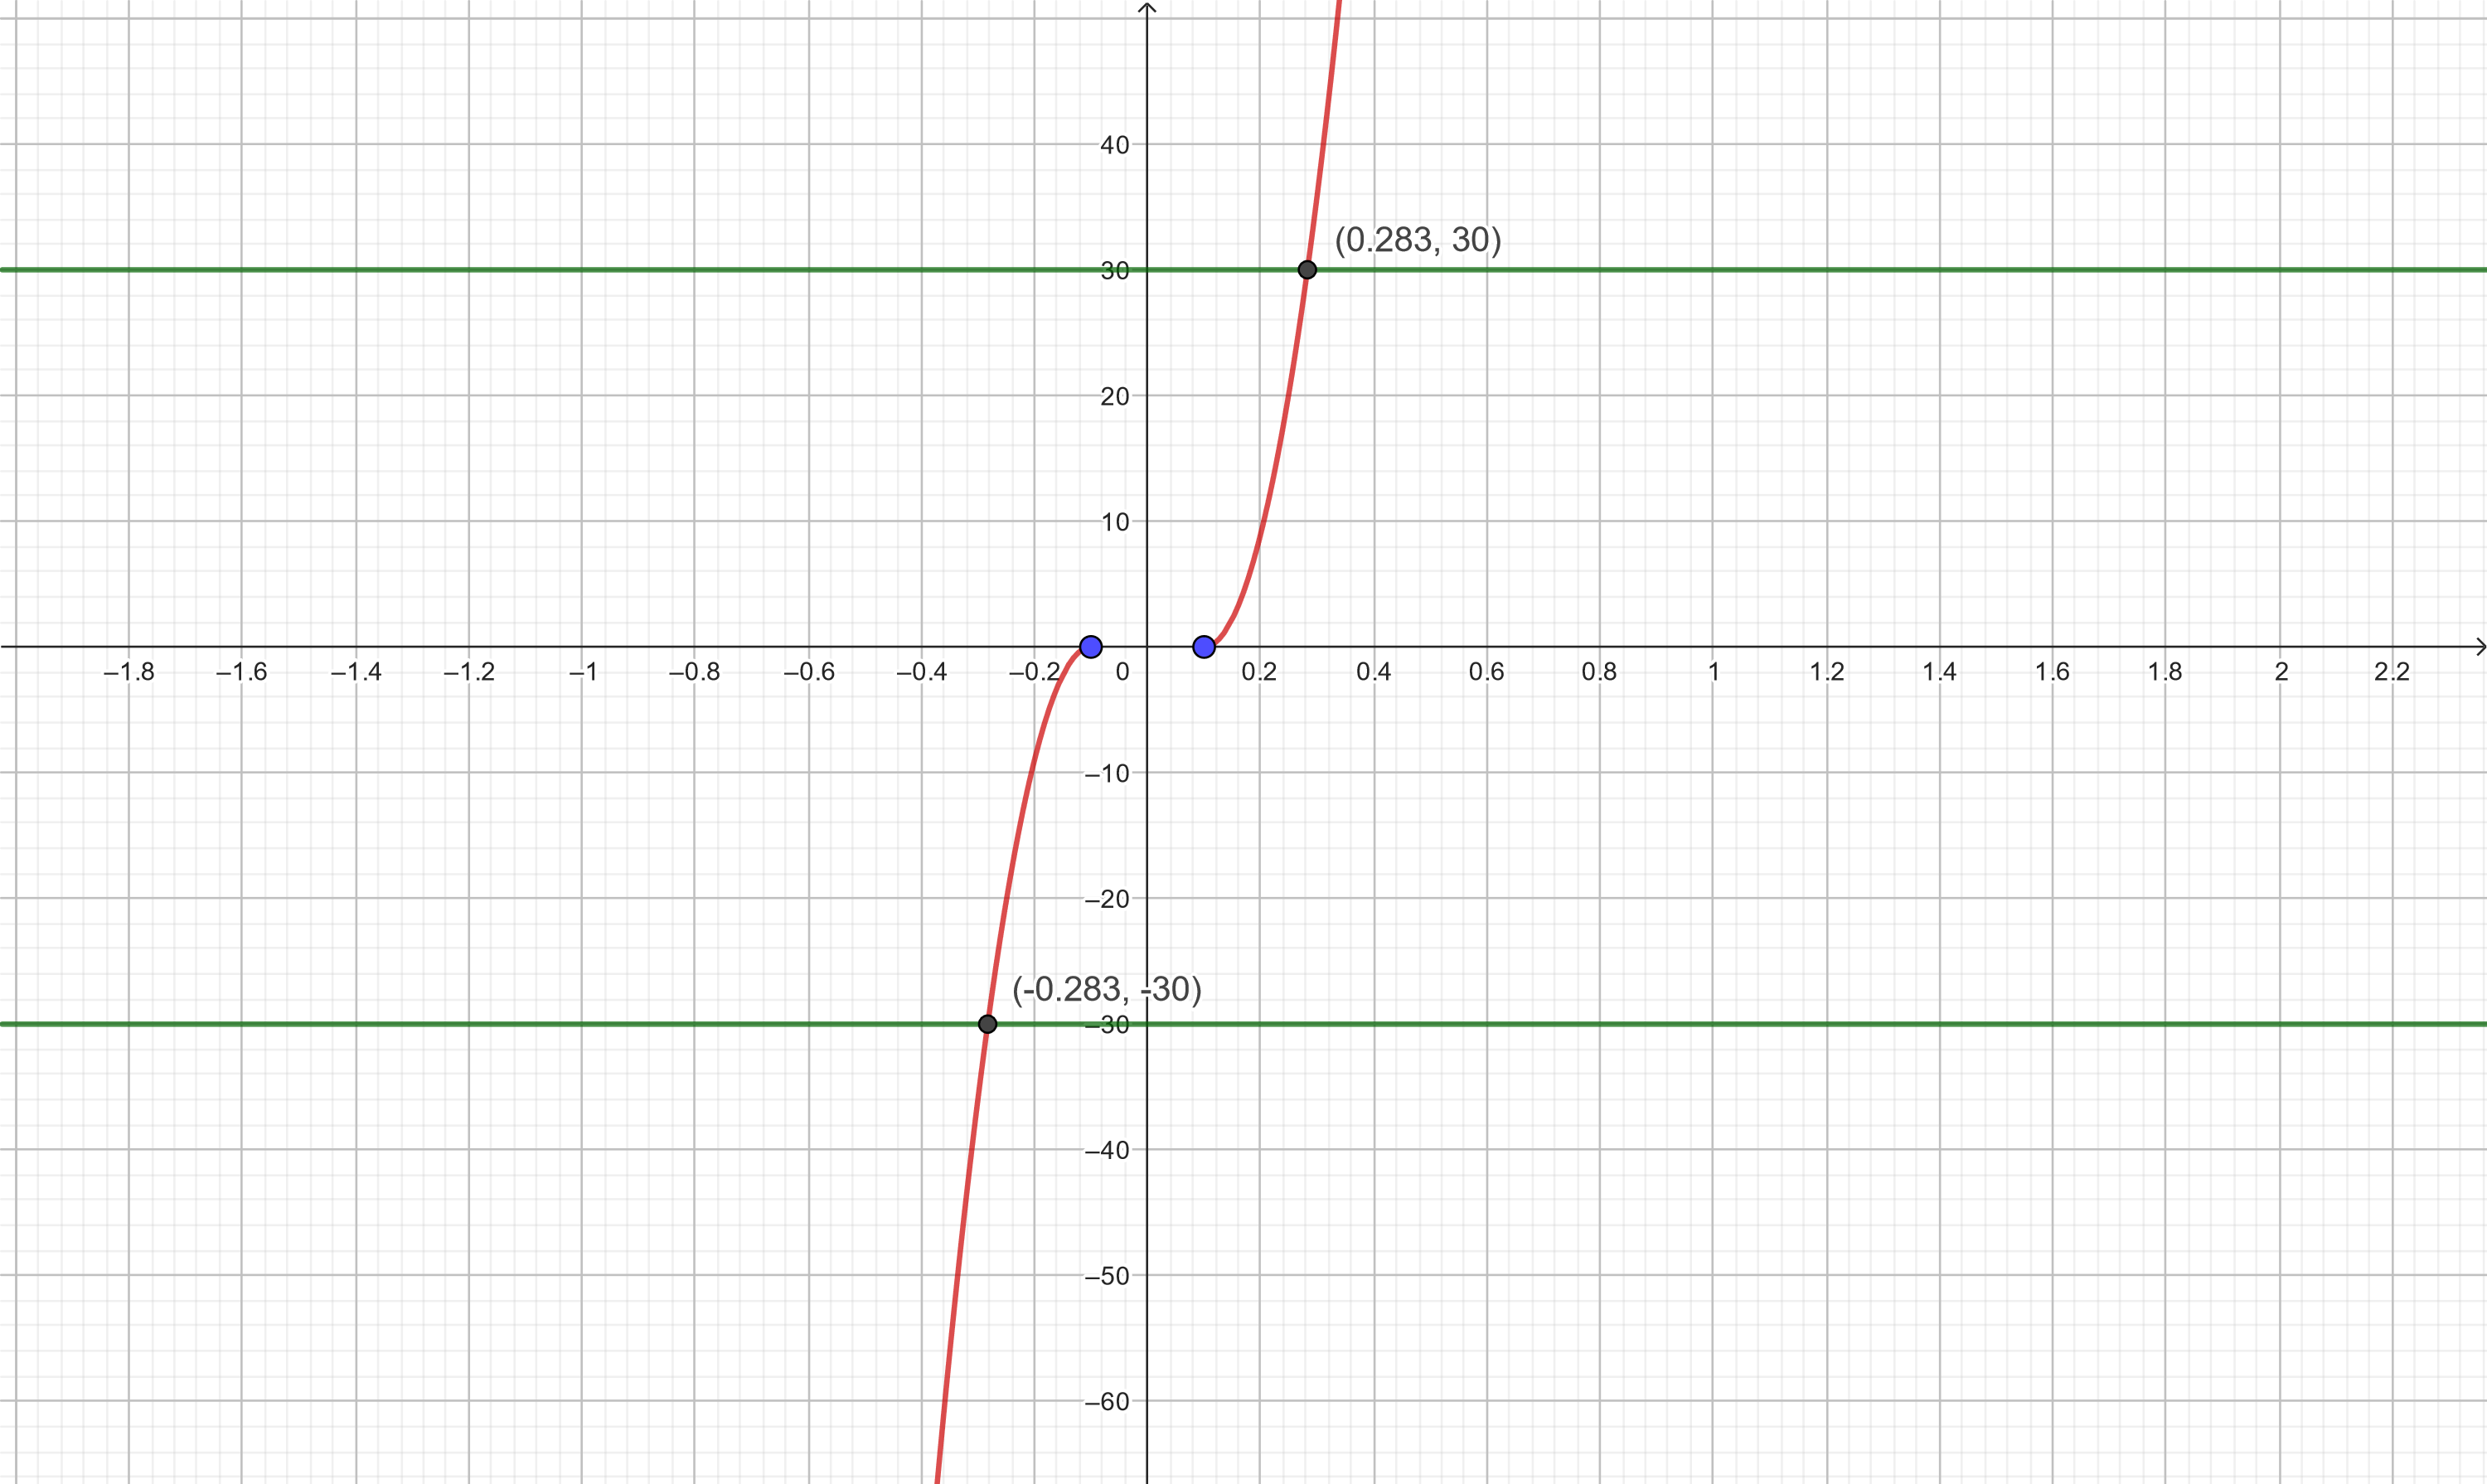
\includegraphics[width=.7\textwidth, keepaspectratio]{img/Rotation}
\caption{Rotation}
\end{figure}
\end{frame}


\begin{frame}{Aufgabe a)}
\begin{figure}
\begin{itemize}
\item Fahre in der Mall und kaufe die 4 Items auf der Liste
\item 2 Items befinden sich unten, 2 oben
\end{itemize}
    \centering
    \movie[externalviewer]{
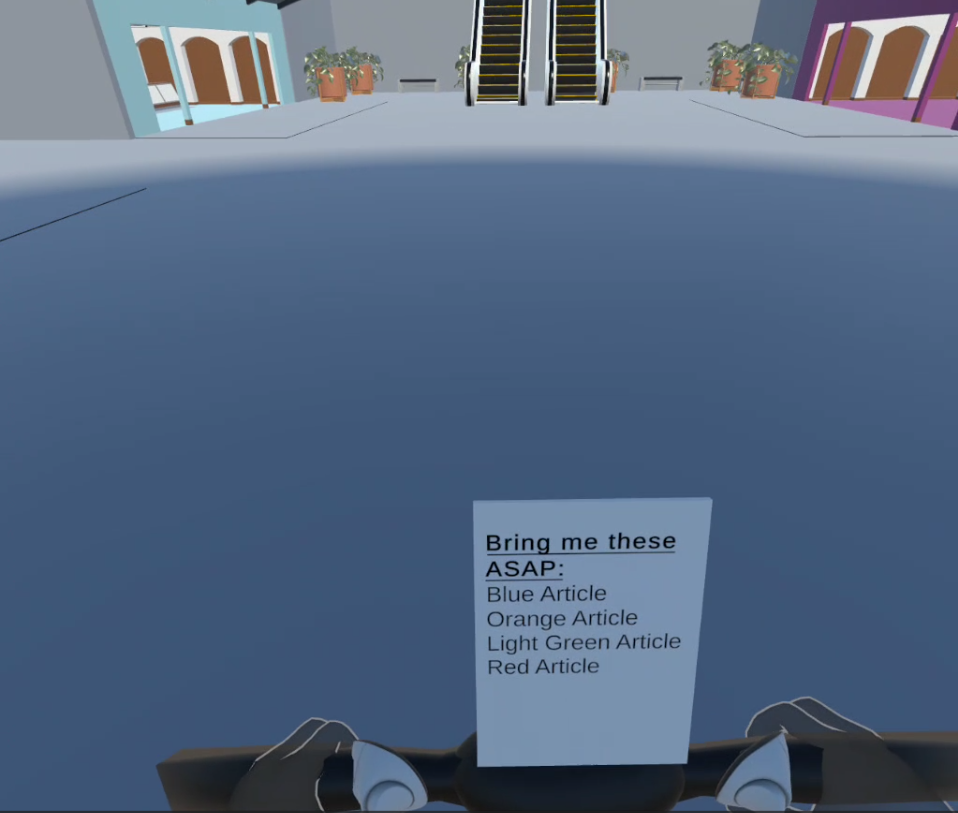
\includegraphics[width=0.6\textwidth, keepaspectratio]{img/aufgabe}
}{vid/Aufgabe.mp4}
\caption{Mallfahrt}
\end{figure}
\end{frame}

\begin{frame}{Aufgabe a) Performance}
\begin{minipage}[c]{0.72\textwidth}
\begin{itemize}
\item Movement bedienbar
\item Aufgabe kann schnell gelöst werden
\item Rolltreppe als kurze Ruhepause
\item Nutzerfreiheit (außer auf der Rolltreppe)
\item Rotation war zu schnell (45°/s -> 30°/s)
\end{itemize}
\end{minipage}
\hfill
\begin{minipage}[c]{0.25\textwidth}
\begin{figure}
\centering

\includegraphics[width=\textwidth, keepaspectratio]{img/escalatorup}
\caption{\cite{esc}}
\end{figure}
\end{minipage}
\end{frame}

\begin{frame}{Aufgabe b) Wahl des Interfaces}
\begin{minipage}[c]{0.72\textwidth}
\begin{itemize}
\item Uns bekannte Fortbewegung mit Hand und Kopf Steuerung
\item Was plausibles für mehr Immersion und Wiedererkennung
\item Rolltreppe statt Rampe für das Mall-Design
\end{itemize}
\end{minipage}
\hfill
\begin{minipage}[c]{0.25\textwidth}
\begin{figure}
\centering
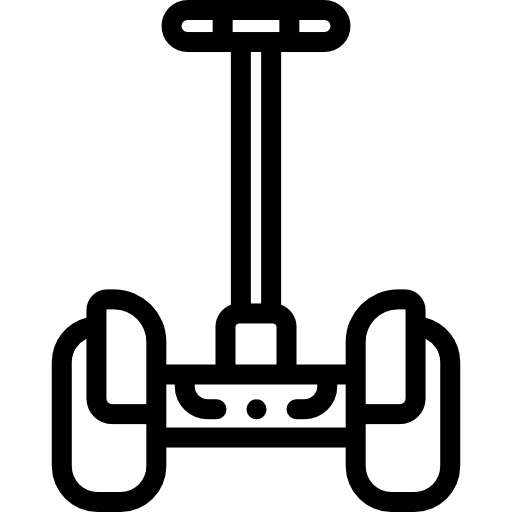
\includegraphics[width=\textwidth, keepaspectratio]{img/segway}
\caption{\cite{segway}}
\end{figure}
\end{minipage}
\end{frame}


\begin{frame}{Aufgabe b) Stärken}
\begin{minipage}[c]{0.72\textwidth}
\begin{itemize}
\item Multimodale Interaktion mit der Lenkstange
\item Immersion durch ein plausibles Szenario
\item Kontrolle der Fortbewegung über Powerfunktion
\item Stoppen der Bewegung über die Deadzone
Präzision
\end{itemize}
\end{minipage}
\hfill
\begin{minipage}[c]{0.25\textwidth}
\begin{figure}
\centering

\includegraphics[width=\textwidth, keepaspectratio]{img/smile}
\caption{\cite{smiley}}
\end{figure}
\end{minipage}
\end{frame}

\begin{frame}{Aufgabe b) Schwächen}
\begin{minipage}[c]{0.72\textwidth}
\begin{itemize}
\item Physische Rotation zerstört das Interface
\item Rotation verursacht trotz Maßnahmen Cybersickness
\item Vertikale Bewegung nur begrenzt möglich
\item Bewegung nicht gut auf höhere Distanzen skalierbar
\item Immersionsverlust durch sich streckende Stange
\end{itemize}
\end{minipage}
\hfill
\begin{minipage}[c]{0.25\textwidth}
\begin{figure}
\centering

\includegraphics[width=\textwidth, keepaspectratio]{img/smileNot}
\caption{\cite{smileyNot}}
\end{figure}
\end{minipage}
\end{frame}


\begin{frame}{Aufgabe b) Messung der Nutzbarkeit}
\textbf{Durchführung einer empirischen Studie zur Usability:}
\begin{itemize}
\item Einkaufsaufgabe durchführen
\item Probanden merken sich wo Artikel gefunden worden
\item Nutzbarkeit über standardisierte Fragebögen (z.B. SUS, NASA-TLX) bewerten
\item Vergleich mit anderen Interfaces (z.B. pointing-based Steering, redirected walking)
\end{itemize}
\end{frame}


\begin{frame}{Aufgabe b) Messung der Performance}
\begin{itemize}
\item Wir messen für jeden Probanden die Zeit
\item Wir loggen die Anzahl der Kollisionen mit Wänden oder anderen Objekten
\item Bei hoher Anzahl an Kollisionen konnte die Umgebung nicht gut wahrgenommen werden
\end{itemize}
\end{frame}


\begin{frame}{Quellen}
	\begin{thebibliography}{1}
\bibitem{esc}[1]{ https://vectorportal.com/de/vector/rolltreppe-nach-oben-vektorzeichen/9123}
\bibitem{segway}[2]{ https://www.flaticon.com/free-icon/segway\textunderscore 1061246}
\bibitem{smiley}[3]{ https://iconmonstr.com/smiley-2-png/}
\bibitem{smileyNot}[4]{ https://iconmonstr.com/smiley-4-png/}
\bibitem{nick}[5]{ Assets: siehe README.txt}
\end{thebibliography}
\end{frame}


	
    	
    	
    	
\end{document}
